\chapter{Introduction}
\label{ch:Intro}
In the recent arena of parallel architectures (multi-cores,
GPUs, etc.), software side lags behind hardware. This is due to the reason that dealing with 
parallelism adds a new dimension to the design of programs, therefore 
makes it complex. One approach for efficient parallelization of programs is to explicitly 
induce parallelism. It includes designing of concurrent programming languages like Go, X10 etc., 
libraries, APIs like POSIX, OpenMP, Message 
Passing Interface(MPI) etc. The main advantage of such approach is that it gives simple and clear directions to the 
compiler to parallelize the code. But the main drawbacks of such approach is that the degree of parallelism totally depends upon 
the efficiency of programmer and imposing external parallelism turns the code into legacy one. 
The other approach is to automatically 
parallelizing sequential programs by compiler which extract parallelism 
without violating correctness. This is a key step in increasing
the performance and efficiency. 
%
\section{Motivation}
Over the past years, lot of work has been done on automatically 
parallelizing sequential programs. These approaches have mainly 
been developed for programs having only static data structures 
(fixed sized arrays) and written in languages such as FORTRAN
~\cite{Allen87automatic,Banerjee93automatic,Wolf91loop,
  Kennedy01Optimizing}. Almost all programming languages
today use the heap for dynamic recursive data structures. 
\begin{comment}
The basic building block of such structure is node which consists 
of one or more fields. Each field is designated as a scalar field or 
pointer field. A pointer field contains either \emph{null} value or pointer to 
a node of the same type. 
\end{comment}

Therefore, any parallelization must also take into account the data
dependency due to the access of common heap nodes of such 
structures. Finding parallelism in sequential programs written
in languages, with dynamically allocated data structures, such
as C, C++, JAVA, LISP etc., has been less successful. One of
the reason being the presence of pointer-induced aliasing,
which occurs when multiple pointer expressions refer to same
storage location. Compared to the analysis of static and
stack data, analyzing properties of heap data is challenging
because the structure of heap is unknown at compile time. It
is also potentially unbounded and the lifetime of a heap
object is not limited by the scope that creates it. As a
consequence, properties of heap (including dependence) are
approximated very conservatively. The approximation of the
heap data dependence information inhibits the parallelization. 

The objective of our analysis is to detect both coarse-grained parallelism 
in the context of function calls, loops and fine-grained parallelism in the 
context of statements. We show the following two examples as motivating 
examples of our work.
\begin{figure}[t]
  \begin{center}
  
    \scalebox{.85}{\begin{tabular}{ c | c }
%    \hline
 	& \multirow{3}{*}{ {\tt
\begin{program}{0}
%  \FL\ \ldots
  \UNL{0} void treeAdd(tree t) \{
  \UNL{1}  if(t == NULL)
  \UNL{2} return;
  \NL{1}     tl = t$\rightarrow$left;
  \NL{1}     treeAdd(tl);
  \NL{1}     tr = t$\rightarrow$right;
  \NL{1}     treeAddd(tr);
  \UNL{1}	t\rtarrow{num} = tl\rtarrow{num} + tr\rtarrow{num};
  \UNL{0} \}
\end{program}
}} \\
%    & \\
      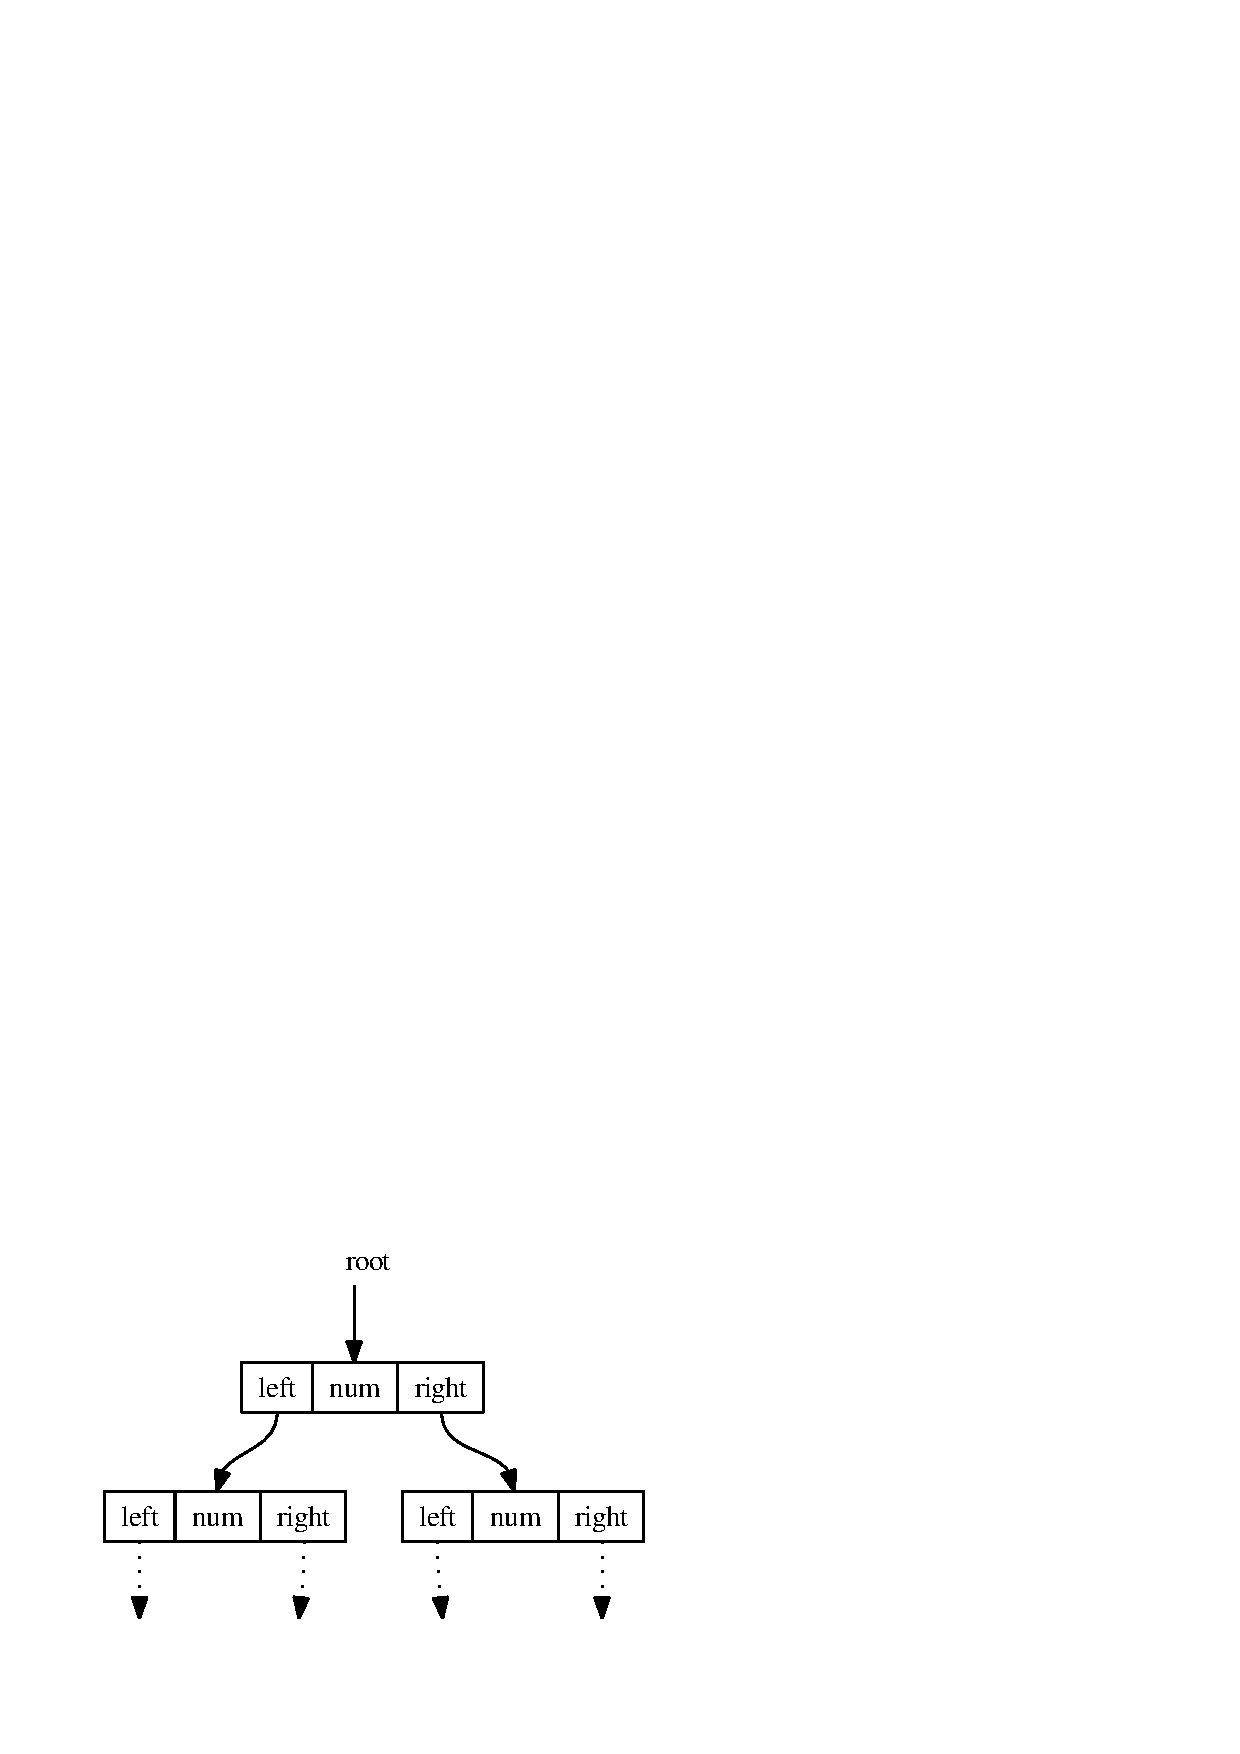
\includegraphics[scale=0.6]{tree_grph}
      & \\
%      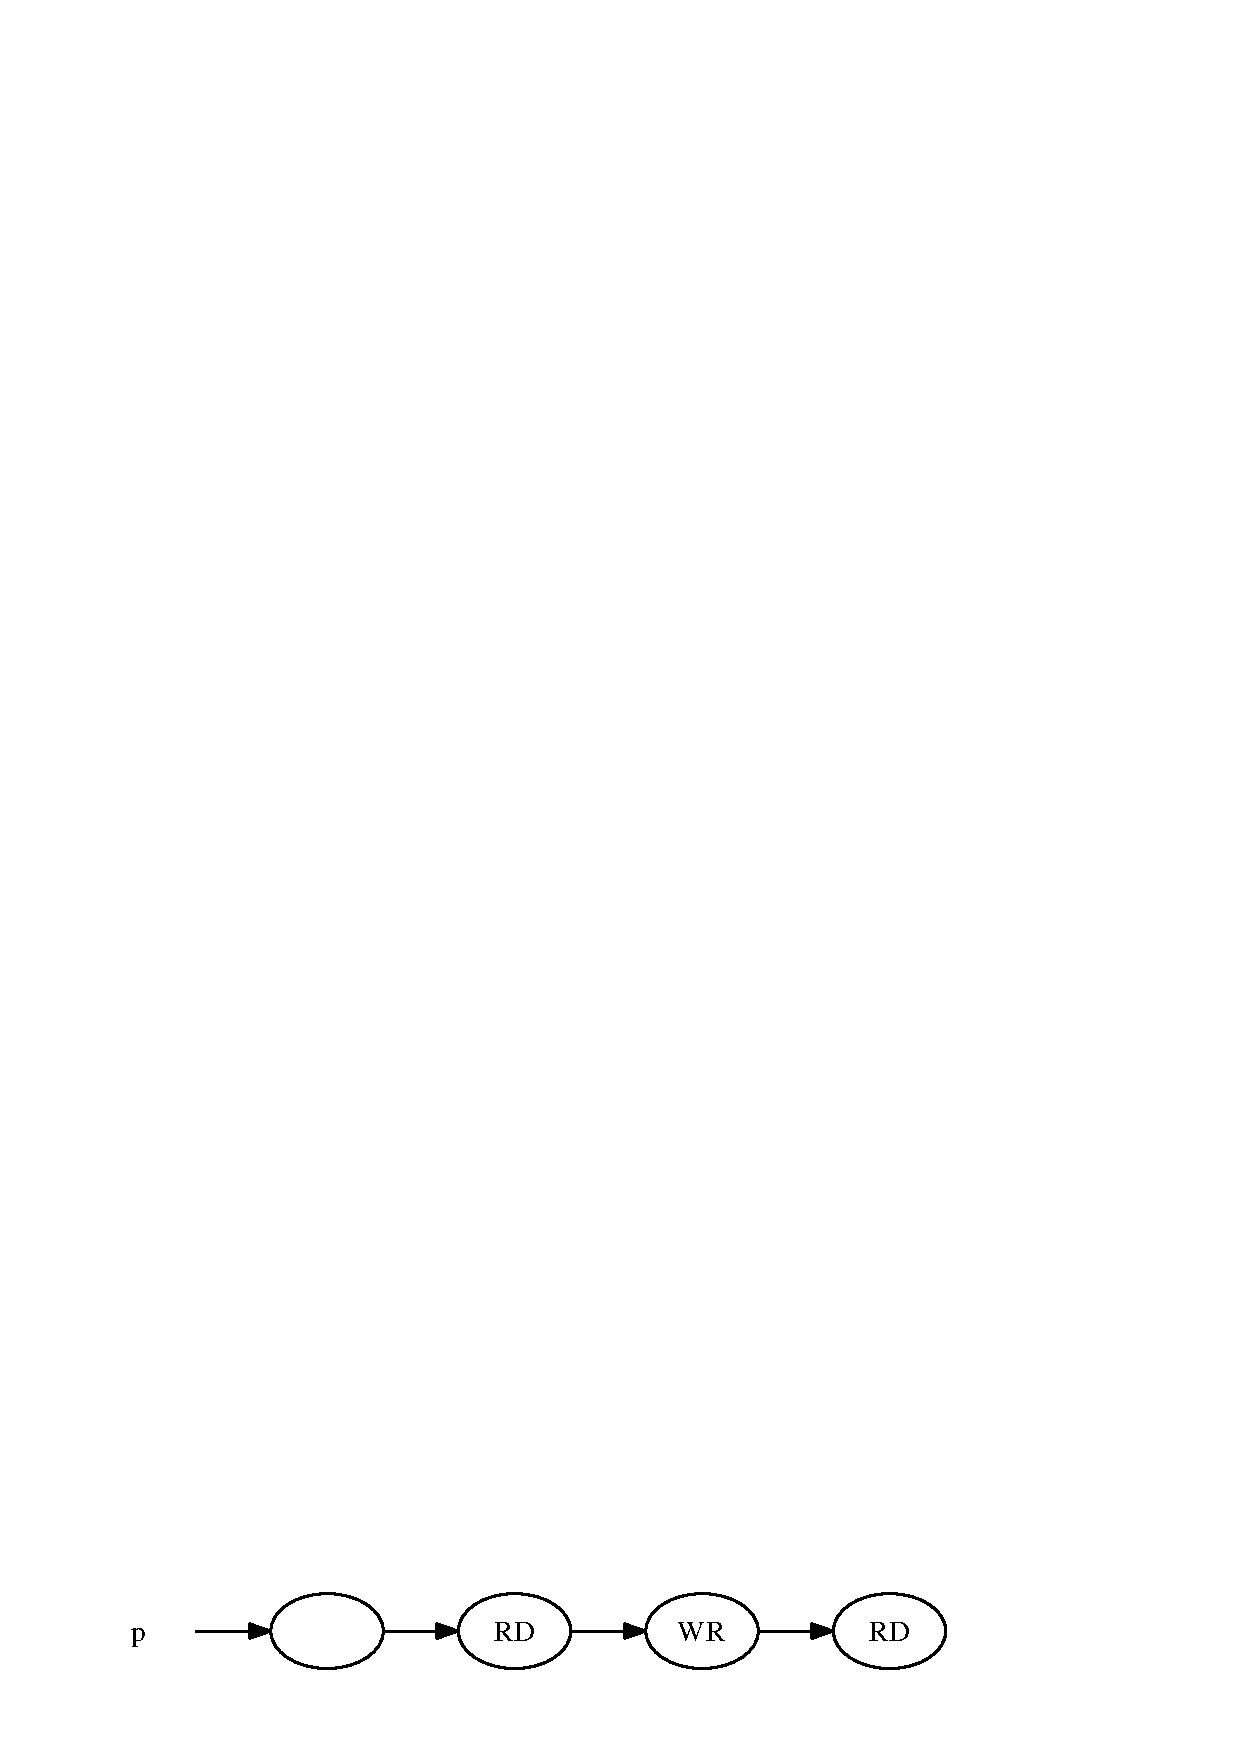
\includegraphics[scale=0.6]{grph_motiv} & \\
%      (a) & (b) \\
     (a) Data structure & 
     (b) Function traversing the data structure. \\
%    \hline 
    \end{tabular}}
  \end{center}
  \hrule
  \caption{\label{fig:motiv1} Motivating example: function-call parallelization}
%\hrule
\end{figure}
\begin{example}{\rm 
Consider Figure~\ref{fig:motiv1} which gives a motivational 
example for parallelism in the context of function calls. It shows 
the tree data 
structure and the function \emph{treeAdd} traversing on the 
data structure. In the code fragment the two calls to the function 
\emph{treeAdd} respectively perform the additions of left and right 
subtrees recursively. If the analysis can ensure that the two function calls 
do not access any common region of heap, they can be executed in parallel.
} 
\hfill\psframebox{}  
\end{example}
%%%%%%%%%%%%%%%%%
\begin{figure}[t]
  \begin{center}
  
    \scalebox{.85}{\begin{tabular}{ c | c }
 %   \hline
      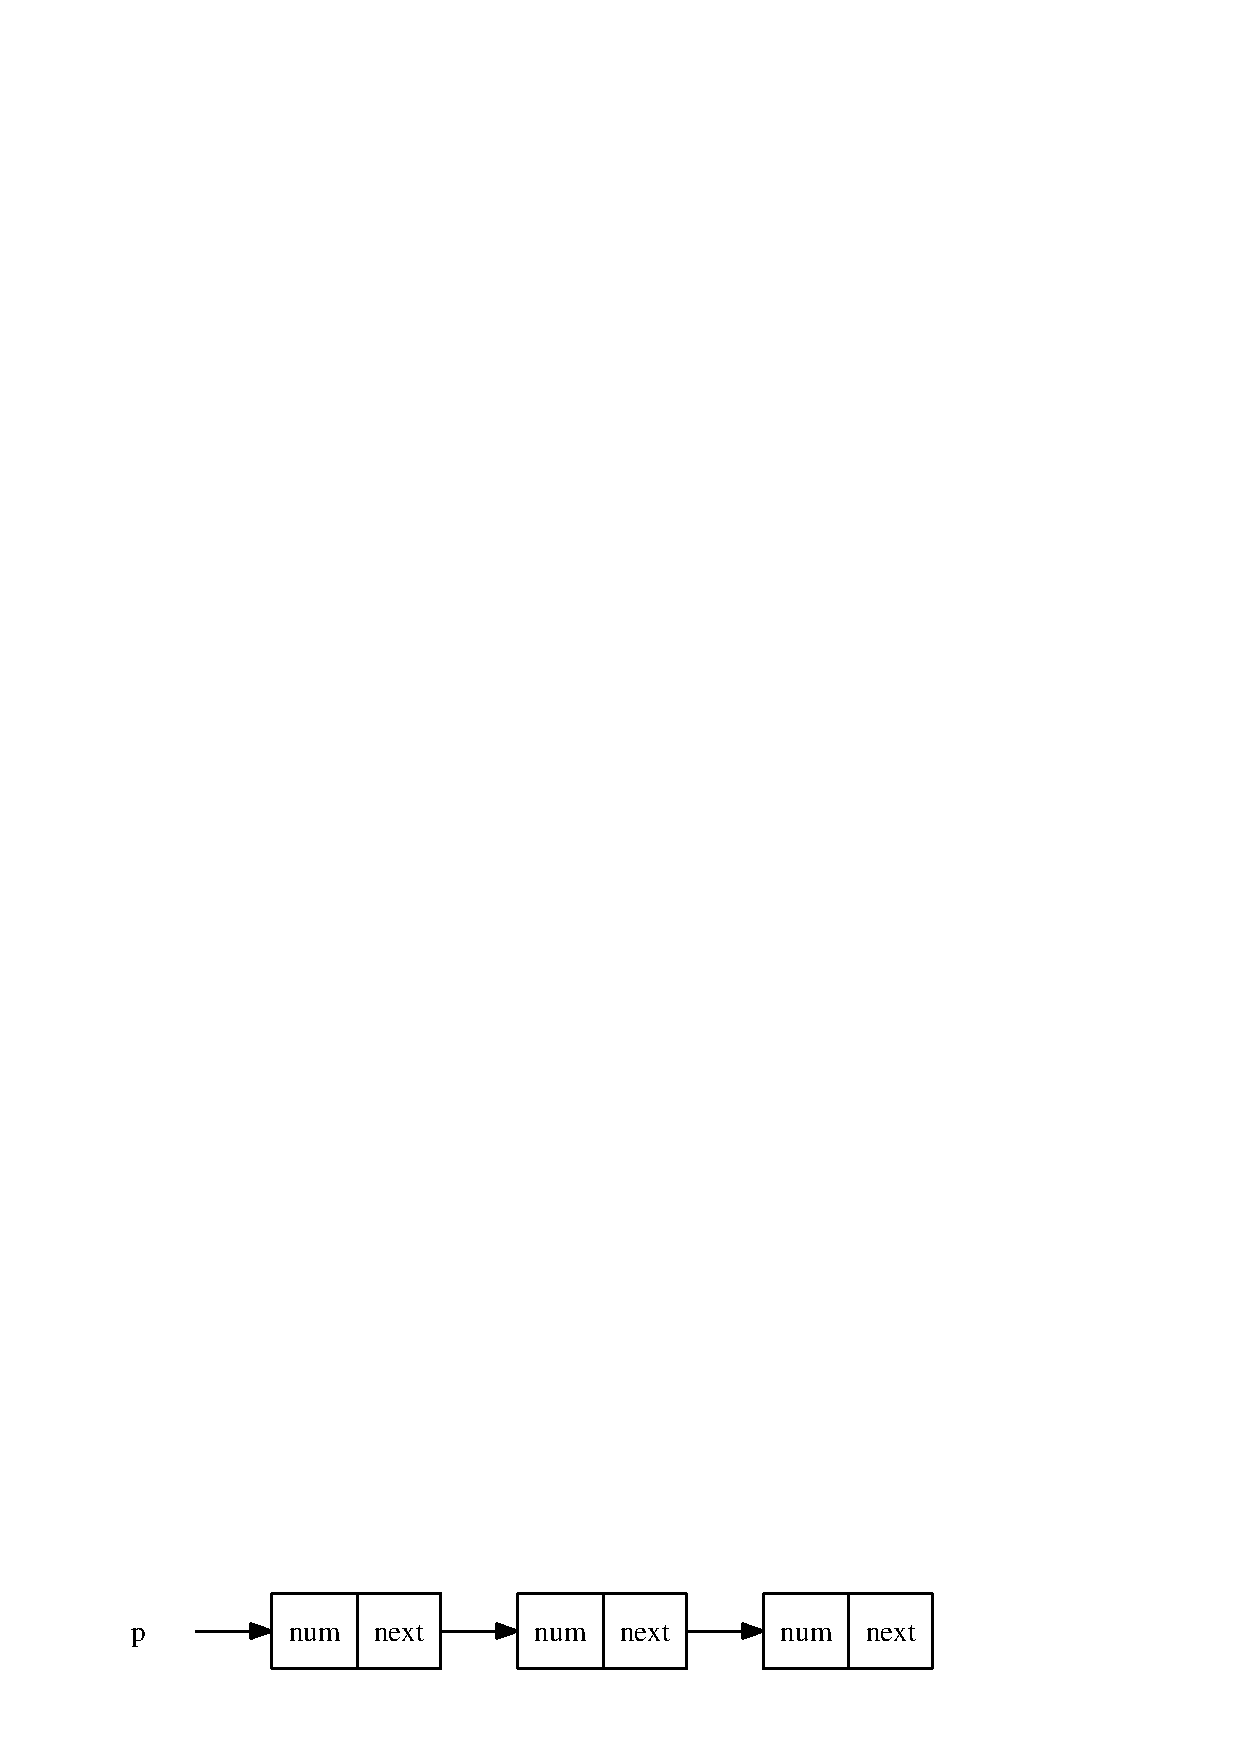
\includegraphics[scale=0.6]{grph4} %\cline{1-1}
      &
      {\tt
\begin{program}{0}
  \FL\ \ldots
  \NL{0} p = list;
  \UNL{0} \WHILE (p$\rightarrow$next != NULL) \{
  \NL{1}     q = p$\rightarrow$next;
  \NL{1}     temp = q$\rightarrow$num;
  \NL{1}     r = q$\rightarrow$next;
  \NL{1}     r$\rightarrow$num = temp;
  \NL{1}     p = r;
  \UNL{0} \}
  \UNL{0} \ldots
\end{program}
} \\
      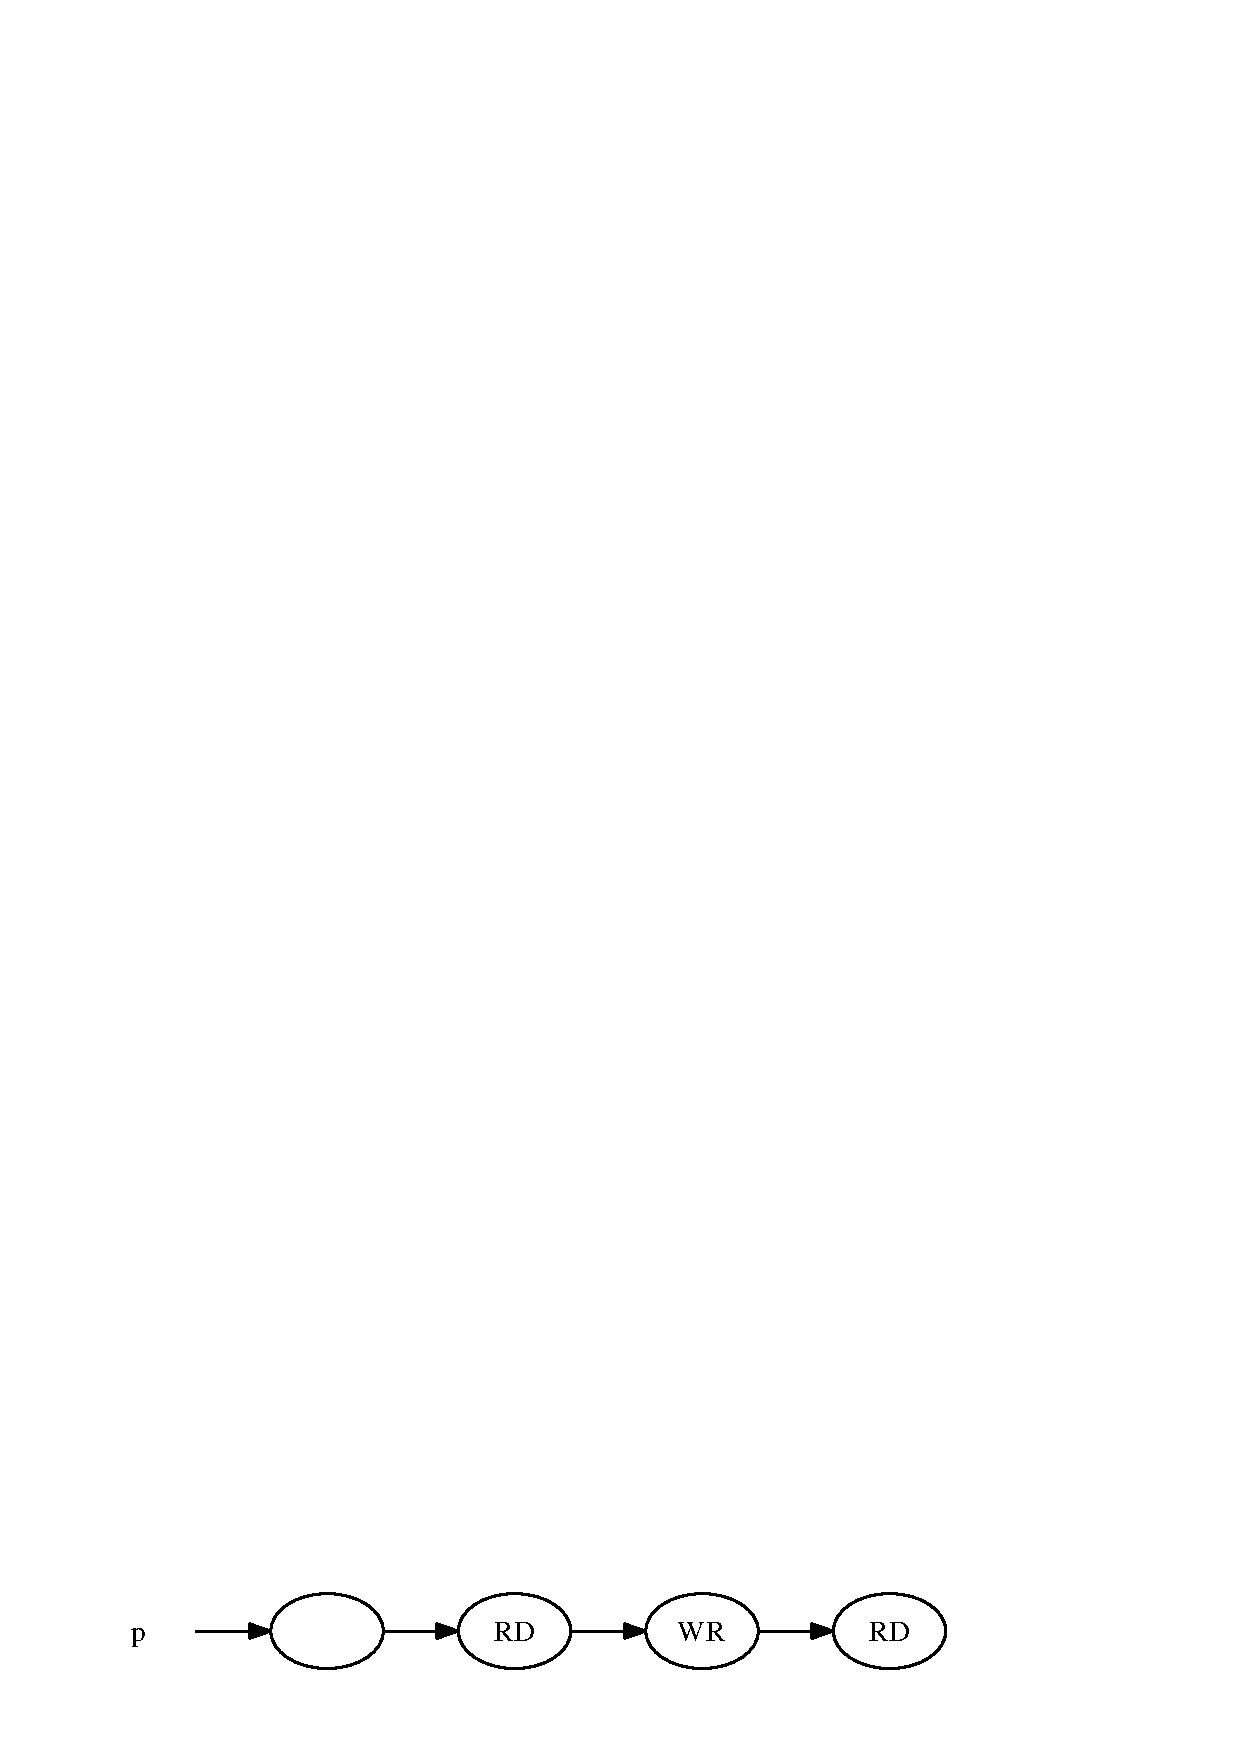
\includegraphics[scale=0.6]{grph_motiv} & \\
%      (a) & (b) \\
     (a) Nodes read and written by code & 
     (b) Loop traversing the data structure. \\
    \end{tabular}}
  \end{center}
  \hrule
  \caption{\label{fig:motiv} Motivating example: loop parallelization}
%\hrule
\end{figure}
\begin{example}{\rm
  Figure~\ref{fig:motiv}
  shows an example of loop level parallelism. It shows list data structure and the nodes of the structure being read and written, tagged by \emph{Read} (\ttf{RD}) 
  and \emph{Write} (\ttf{WR}) access by the code fragment traversing the
  data structure. Note that, the first node of the structure is a special node which is neither 
  read nor written by the code fragment. The performance of the code can be improved if the loop can
  be executed in parallel. However, without the knowledge of
  precise heap dependences, we have to assume worst case
  scenario, i.e.,  the  location read by the statement {\tt
    S3} in some iteration could be the same as the location
  written by the statement {\tt S5} in some other iteration.
  In that case,  it is not possible to parallelize the loop.
 
  Our dependence analysis can show that the locations read by
  {\tt S3} and those written by {\tt S5} are mutually
  exclusive. Further, it also shows the absence of any other
  dependences.  This information, along with the information
  from classical control and data dependence analysis, can be
  used by a parallelizing compiler to parallelize the loop.
}
\hfill\psframebox{}  
\end{example}

This report explains our approach for a practical heap data dependence analysis. 
As it is understood that we are only talking about data dependences, we drop the term 
data in the rest of the report. 
%
\section{Contributions of our Work}
Our work contributes in the area of heap based 
dependence analysis. We present a novel approach 
which identifies dependences and extracts parallelism for a sequential program. 
In particular, our approach finds out dependences between two statements. 
This enables us to find out whether two procedure calls 
access disjoint structures, hence can be executed in parallel. 
Then we refine this technique to work better 
in presence of loops. We also extend the work of loop analysis 
for static and scalar data to support heap intensive loops.

\section{Organization of the Thesis}
The rest of the thesis is organised as follows. We discuss about related 
work done in the field of heap intensive dependence analysis in Chapter~\ref{ch:RelatedWork}.
Chapter~\ref{ch:back} specifies the imperative programming model 
for which our analysis is defined and gives the other background 
details. Chapter~\ref{ch:dep} through~\ref{ch:interdep} provide a complete 
description of our practical dependence analysis applied to 
dynamically allocated structure. Chapter~\ref{ch:dep} gives the detailed 
explanation of the intra-procedural dependence detection technique 
which separately works on each procedure of a program. Chapter~\ref{ch:loopdep} 
presents our method to handle loops in a more specific way. We also 
give the inter-procedural framework for our analysis in Chapter~\ref{ch:interdep}. 
Chapter~\ref{ch:result} demonstrates our whole method by extensively 
analysing few benchmark codes. We conclude the report in Chapter~\ref{ch:conclusion} 
by giving the direction for future research.